\chapter{Traveling Ionospheric Disturbances}

\section{Introduction}
Travelling Ionospheric Disturbances (TIDs) are wave-like plasma oscillations in the ionosphere which can occur at different temporal and spatial scales. TIDs are understood to be the ionospheric manifestation of Atmospheric Gravity Waves (AGWs) via ion-neutral coupling in the Ionosphere-Thermosphere (IT) system \citep{hines_1960}. TIDs with wavelengths less than a 100 km are classified as Medium Scale TIDs (MSTIDs) and can be caused by various processes, but in general are associated with tropospheric forcing. TIDs with wavelengths larger than 1000 km and a with time period of greater than one hour are classified as Large Scale TIDs (LSTIDs) \citep{hocke1996review}.

Most LSTIDs propagate from either pole and are associated with magnetic disturbances. Geomagnetic storms cause rapid enhancement of the auroral electrojet that leads to thermospheric heating and expansion \citep{davis_polar_1971,chimonas_atmospheric_1970}. This generates AGWs that propagate towards the equator. The divergence of AGWs in turn generates LSTIDs \citep{prolss_lstid_2000}. LSTIDs that have propagated equatorward and are associated with geomagnetic storms have been observed by previous studies (see \citet{habarulema_storm_tid}, and references therein). For example, based on magnetometer measurements, \citet{habarulema_storm_tid} showed that poleward TIDs were launched following southward turning of the Interplanetary Magnetic Field (IMF).

In addition to geomagnetic storms, solar eclipses are also known to produce AGWs (\citet{liu_1998, chimonas1970}, etc.) and leave the upper atmosphere disturbed. For example, \citet{coster_gnss_2017}, based on Total Electron Content (TEC) measurements, saw enhanced TEC structures along the Rocky mountains as the shadow of the eclipse passed over. \citet{goncharenko_mh_hill_eclipse}, based on digisonde and ISR measurements of ionospheric parameters at Westford, MA ($\sim$ 60\% peak obscuration), observed fast (20-40 m/s) upward plasma drift above the HmF2 immediately following the maximum obscuration. Neutral wind velocity derived by using the OI 630.0 nm (red line) emission measurements by a Fabry-Perot Interferometer (FPI) in Brazil showed perturbation in neutral winds far from the path of the eclipse. Global-scale simulations using a UV obscuration mask that mimics the eclipse's effect on the upper atmosphere successfully predicted the measured changes in neutral wind qualitatively \citep{harding_nightside_eclipse}.

% The 2017 solar eclipse occurred over the continental USA where numerous satellite receiver and ground based instruments were present, leading to abundance of data for studying the effects on the upper atmosphere. Some of the studies have already resulted in observation of unexpected phenomenon. \citet{coster_gnss_2017}, based on Total Electron Content (TEC) measurements, saw enhanced TEC structure along the Rocky mountains as the eclipse passed through them. Based on differential TEC (dTEC) measurement and EUV occultation map, \citet{mrak_eclipse_2018}, found that the large-scale perturbation structure in dTEC immediately following the eclipse mimicked the gradient of the EUV map. This led them to theorize that the perturbation seen in TEC was a directly a consequence of EUV modulation during the eclipse not AGW's.

On August 22, 2017 a TID event following a minor geomagnetic storm (minimum DST index $\sim$ -30 nT, peak Auroral Electrojet index $\sim$ 1000 nT) was observed. The geomagnetic storm followed the eclipse of August 21, 2017 hours earlier (8 hours at Carbondale, IL). In this paper, based on ground-based airglow measurements, GPS based Total Electron Content (TEC) measurements, and ionospheric parameters derived using digisonde measurements we analyzed the TID event and characterized its wave properties. The dominant time period in all of these measurements was $\sim$ 1-1.5 hours. Furthermore, based on the Global Ionosphere-Thermosphere Model (GITM) estimation, preconditioning due to the eclipse seems to have enhanced the effects of the observed TIDs.
\section{Data}
\subsection{Spectral Data}
Our observation of the TIDs from Carbondale, IL (Geographic location: 37.7$^\circ$N, 89.2$^\circ$W)  were made using the High Throughput and Multi-slit Imaging Spectrograph (HiT\&MIS) \citep{hitmis}. HiT\&MIS can simultaneously measure six upper atmospheric emission features at high resolution ( $\sim$ 0.02 nm/px in red line for example). The field of view (FOV) of HiT\&MIS is approximately 0.1$^\circ$ by 50$^\circ$ and was centered at an elevation angle of 45$^\circ$ looking towards the northwest (Figure \ref{fig:elayer}). The spectral images were recorded at a cadence of 4 minutes using a PIXIS CCD from $\sim$ 0200 UT to 1000 UT August 22, 2017.  Simultaneous measurements in red and OI 557.7 nm (green line) are used for this particular study. 
\begin{figure}
	\centering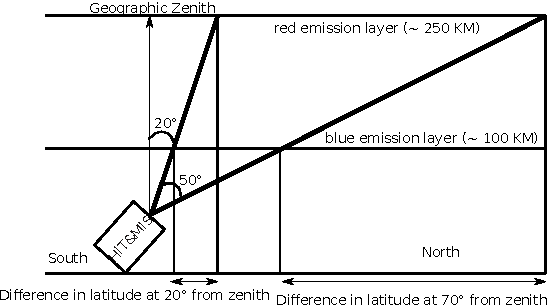
\includegraphics[width=35pc]{elayer.pdf}
	\caption{Viewing geometry of the HiT\&MIS instrument August 21-22, 2017 at Carbondale,IL. The latitudes traced by the red and the green lines are shown assuming the peak emission height of
		250 km and 150 km, respectively. Note that for measurements closer to the zenith, the range of latitudes covered by each emission layer is small. However for measurements far away from the zenith, emission from a larger latitude range are integrated along the line of sight.}
	\label{fig:elayer}
\end{figure}

From the raw CCD image, regions around the red and green line spectrum plus a diagnostic cloud line (also observed by HiT\&MIS ) as a function of HiT\&MIS look direction and wavelength were extracted.  Cloud line is based on measurement of NeI 630.5 nm line (reflection of street lights from clouds) and is used as indicator of cloud activity. The baseline was obtained by linear fitting the spectrum edges. See \citet{aryal_energy} for a more detailed description of spectra extraction using HiT\&MIS.

The data were co-added along the wavelength axis ($\approx$ $\pm$0.3 nm from the line center) to obtain the brightness for the red and green lines as a function of look direction and time.
% Based on the peak emission heights of red (250 km) and the green line (150 km) from the GLobal airglOW (GLOW) model, and the viewing geometry of HiT\&MIS, the look angles are then converted to the latitude (projection of emission height). 
The red and green brightnesses for both the night before (for comparison) and the night of the eclipse (TID event) are presented in Figure \ref{fig:keo_profile}. The red and green line brightnesses on the night with the TID event show wave-like brightness perturbation while the perturbation (especially in green line) only correlated well with the cloud line the night before.
\begin{figure}
 \centering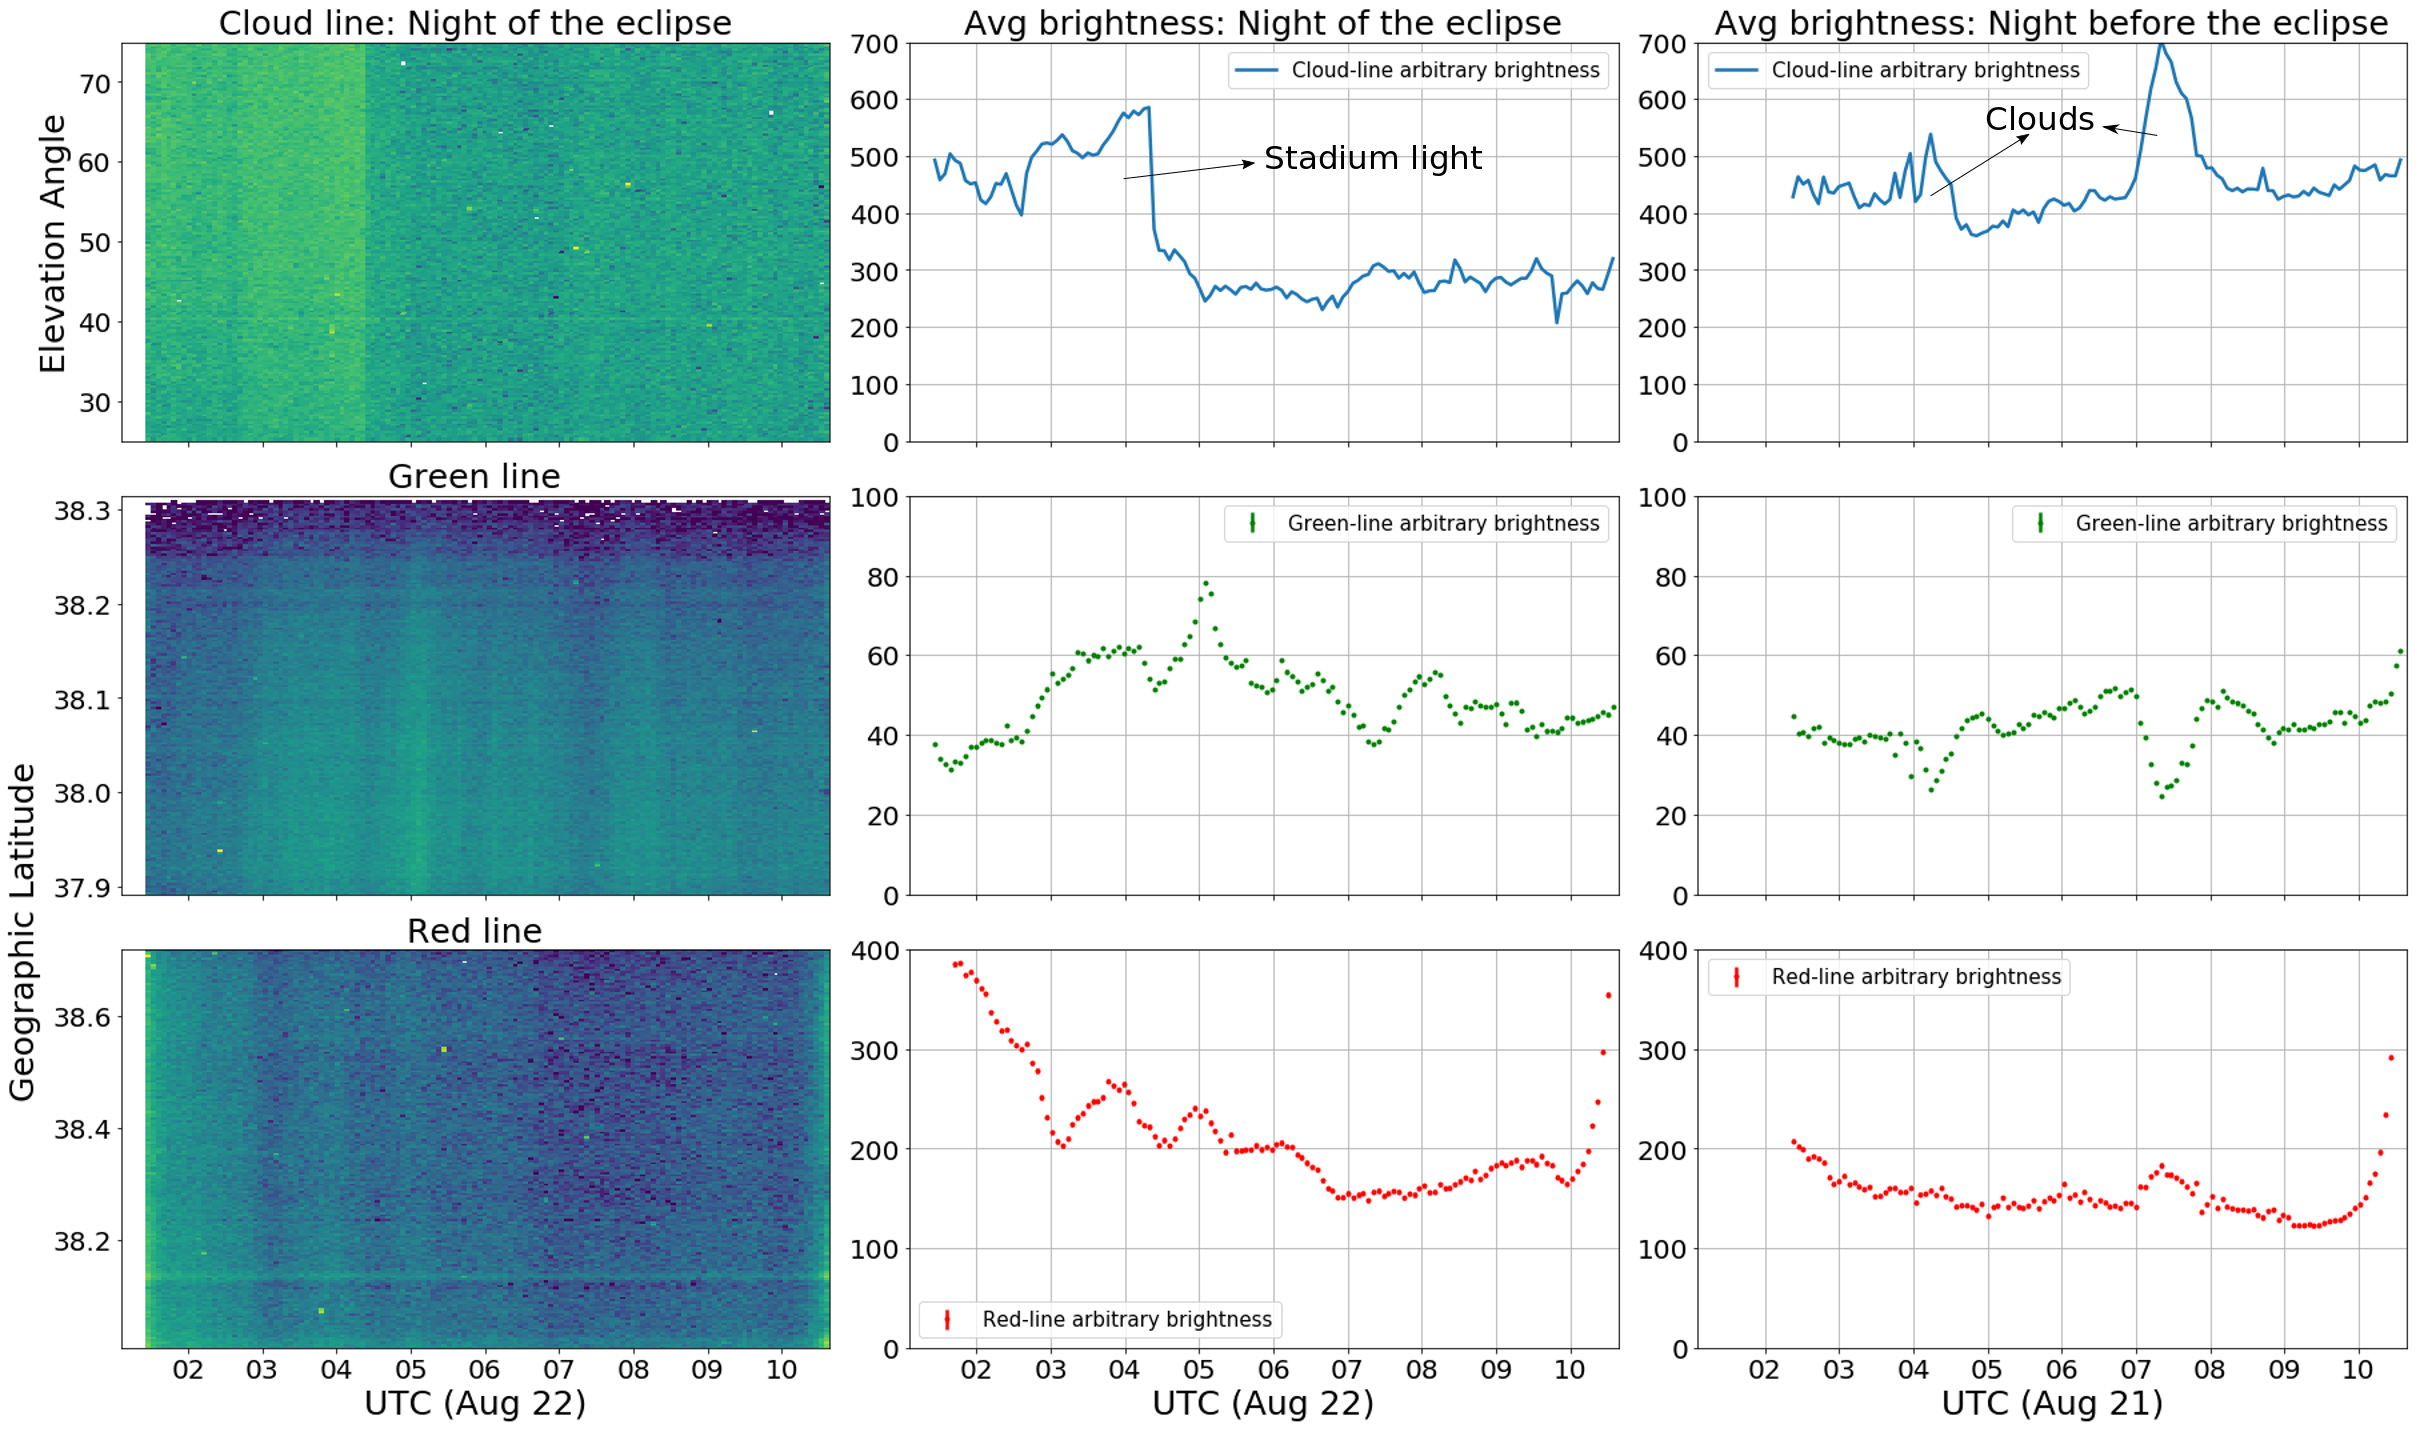
\includegraphics[width=35pc]{car_Aug2122_both.png}
 \caption{Left: Brightness keogram of cloud, red and green lines as a function of look direction (or longitude) on the night of the eclipse. Brighter color represents higher brightness (in arbitrary units).  White-space represents negative values encountered after baseline subtraction. Center: Brightness averaged over the whole field of view for each representative keogram presented on left. Notice clear wavelike perturbation in both red and green lines. Right: Average brightnesses in cloud, red and green lines on the night before the eclipse (keogram not shown).  The dips in the green line coincides with the increase in the cloud line brightness. There is a sudden drop in the cloud line brightness around 0400 UTC, this is due a nearby stadium light in HiT\&MIS FOV being switched off (this effects the cloud line). }
 \label{fig:keo_profile}
 \end{figure}
%Text here ===>>>
\subsection{Differential TEC data}
To validate our observation of the TID-generated brightness perturbations, we looked at satellite-based GPS TEC measurements. [Sebastian's part here a few lines or a paragraph or two on the DTEC processing]
Figure \ref{fig:dtec_carb} shows the Differential Total Electron Content (DTEC) measurements and the dynamic part of the red and the green line profiles at Carbondale, IL. Good correlation is seen between the TEC and the brightness perturbations from after 0300 UTC to 0600 UTC is seen.
[Also, DTEC obtained for the continental USA  (see Supplementary video) shows a series of TEC enhancements and depletion structures propagating equatorward; can decide if we this might be useful to add.]


\begin{figure}
	\centering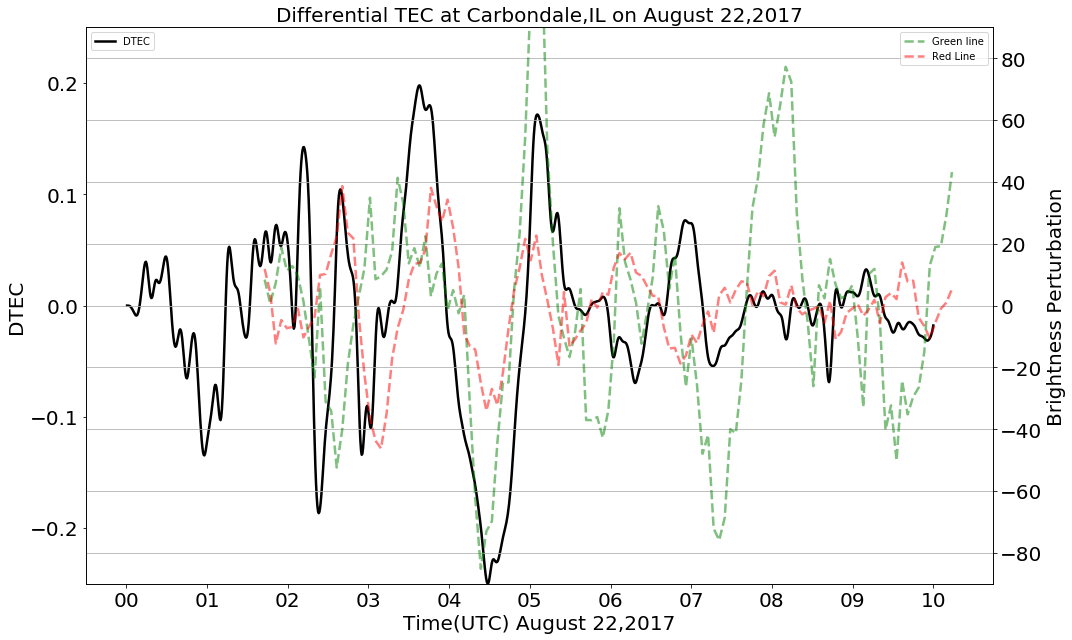
\includegraphics[width=35pc]{aug22_dtec_bper.png}
	\caption{DTEC obtained for Carbondale, IL on August 22, 2017 from GPS TEC measurements.  Notice stronger perturbations starting after 0300 UTC and good correlation (from 0300 - 0600 UTC) with red and the green line profiles  shown in light-red and light-green dashed lines, respectively. }
	\label{fig:dtec_carb}
\end{figure}
%% Sebastian's part
\subsection{Digisonde Data}
% Ivan's part
To study the nature of TIDs we also looked at digisonde-based ionospheric parameters from two locations, Idaho National Lab (INL, 43.5$^\circ$N, 112$^\circ$W), and Millstone Hill (MH, 42.5$^\circ$N, 71.4$^\circ$W). These measurements are from a network of digisonde instruments, known as the Global Ionosphere Radio Observatory (GIRO). The Maximum Usable Frequency (MUF) parameter is used for the current case because it is derived using foF2 (proportional to NmF2) and hmF2  and thus is more sensitive to ionospheric perturbations.
Figure \ref{fig:digi} shows the MUF profiles at MH and INL from 1900 UTC on August 21, 2017 to 0600 UTC August 22, 2017. The MUF profile at both locations are dynamic and the perturbation before the start of geomagnetic disturbances (0000 UTC August 22, 2017) could be associated with the effect of the eclipse.

[Main point: From the observations we conclude that the TID was large scale in nature. Also, periodicity before midnight could be eclipse's effect? See ionospheric fluctuations at far away locations and DTEC data. I have put generic information about MUF need to add more from Ivan.]
   \begin{figure}
 \centering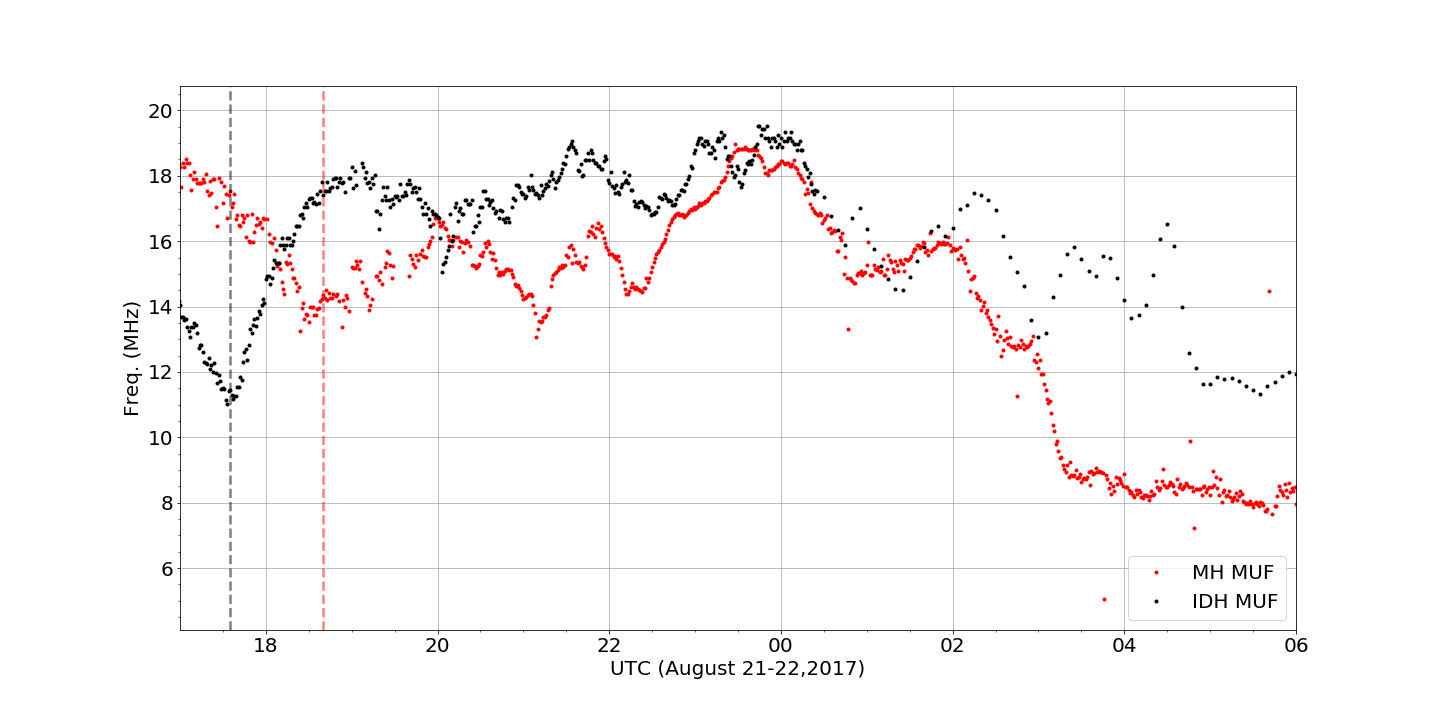
\includegraphics[width=35pc]{digi_muf_21-22.png}
 \caption{Digisonde profiles of MUF  at Idaho National Lab (IDH) and Millstone Hill (MH) from 1700 UTC August 21 to 0600 UTC August 22, 2017. IDH was close to the path of the totality and the  99\% peak obscuration time is shown by dashed-vertical black-line. MH was on the path of partial eclipse and the 60\% peak obscuration time is shown in dashed-vertical red-line. Notice that perturbations occurred at both the locations before midnight UTC (August 22, 2017); these might be associated with after effect of the eclipse. The perturbations after midnight UTC seem to be associated with TIDs generated due to increase in auroral currents.}
 \label{fig:digi}
 \end{figure}
 

\section{Results}

To understand the cause of the AGW and TID observed, we looked at the geomagnetic conditions before and during the measurement times. Figure \ref{fig:gindx} shows the DST and the Auroral Electrojet (AE) indices from 1800 UTC on August 21, 2017 to 1000 UTC on August 22, 2017. DST  index is a measure of the equatorial ring current strength and is evaluated by averaging ground-based measurements of magnetic fields near the equator \citep{kauristie_dst}. The AE index is a measure of the strength of auroral currents and is obtained from geomagnetic measurements near the polar cap.  During the time of the observations presented in this paper, the AE index peaked ($\sim$ 1000 nT) at 0200 UTC on August 22, 2017. Peak deviation in DTEC  occurred right after this peak $\sim$ 0300-0500 UTC on August 22, 2017 (Figure \ref{fig:dtec_carb}). AE strength is directly related to Joule heating of the IT system \citep{ae_joule} which in-turn could potentially lead to poleward propagating TID. Thus, we conclude that the observed TIDs (and AGWs) were generated by geomagnetic effects that induced changes in the auroral current leading to rapid heating and expansion of the thermosphere. 
%%%geomagnetic index plots
   \begin{figure}
 \centering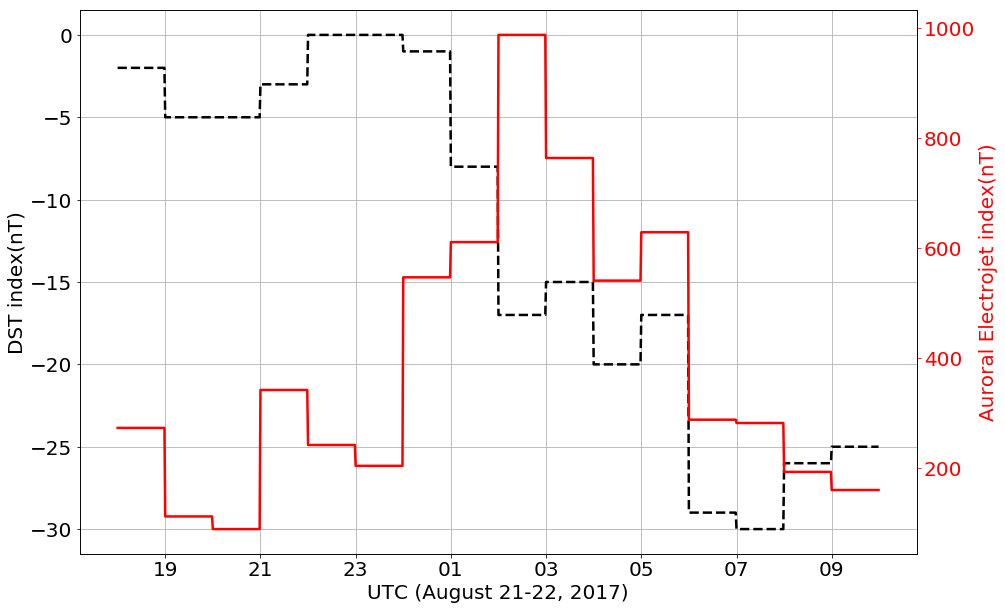
\includegraphics[width=30pc]{tid_geindex.png}
 \caption{DST and Auroral Electrojet (AE) indices before and during HiT\&MIS observation times. Note increase in AE starting midnight UTC on August 22, 2017. AE index is a measure of strength of auroral currents, thus increase in AE represents increase in Joule Heating in auroral (polar) ionosphere that heats and rapidly expands the thermosphere leading to AGWs. }
 \label{fig:gindx}
 \end{figure}
 %%%%%%%%
 
\subsection{Wave Characteristics}
 We performed wavelet analysis on red and green line brightness profiles (Carbondale, IL) , digisonde MUF profiles (at Idaho National Lab and Millstone Hill locations), and DTEC obtained from GPS measurements (Carbondale, IL). Wavelet analysis has been used by previous studies to study wave characteristics of AGWs and TIDs \citep{singh_effect_2016,wvlt_B} . For example, \citet{singh_effect_2016} studied the vertical propagation of AGWs  due to cyclone Nilofer by performing wavelet analysis optical emission brightnesses originating at different altitudes.
 
Our wavelet analysis is based on the guide presented in \citet{torrence_wavelet} and implemented using the waipy package on python (https://github.com/mabelcalim/waipy). Averaged red and green line brightnesses were used  as there were no significant change in dynamic behavior as a function of look direction (or latitude, see Figure \ref{fig:keo_profile}). The brightnesses and the MUF profiles were subtracted with a polynomial fit of themselves to obtain only the dynamic part of the profiles. The DTEC is the dynamic part of the TEC measurement and its extraction is described in earlier section. These dynamic profiles were then normalized (zero-mean, unit variance normalization) and the analysis was performed on these normalized values. 
 
The wavelet spectra for the red and the green lines, shown in Figure \ref{fig:red_green_wv}, reveal a dominant time period of 1.2 hours for the red line and 1.6 hours for the green line. However, the wavelet power for the red line peaked around 0200 UTC and the green line wavelet power peaked around 0600 UTC. The MUF wavelet spectra for both locations show similar dominant time period of around 1 hour (plus others) with peaks at two different times (Figure \ref{fig:muf_wv}). The time period of 1 hour prior to midnight UTC could be the after effect of eclipse as the perturbations precede geomagnetic disturbances. The DTEC wavelet spectra showed a dominant time period of 1.7 hours peaking around 0400-0500 UTC.  It is to be noted that the MUF is sensitive to the bottom-side ionospheric plasma densities, the red and green line brightnesses are sensitive to both the plasma and the neutral densities at the altitude they peak at, and the TEC measurements are sensitive to the topside ionospheric plasma density. This could explain why the dominant time period differ slightly for these measurements.
\begin{figure}
 \centering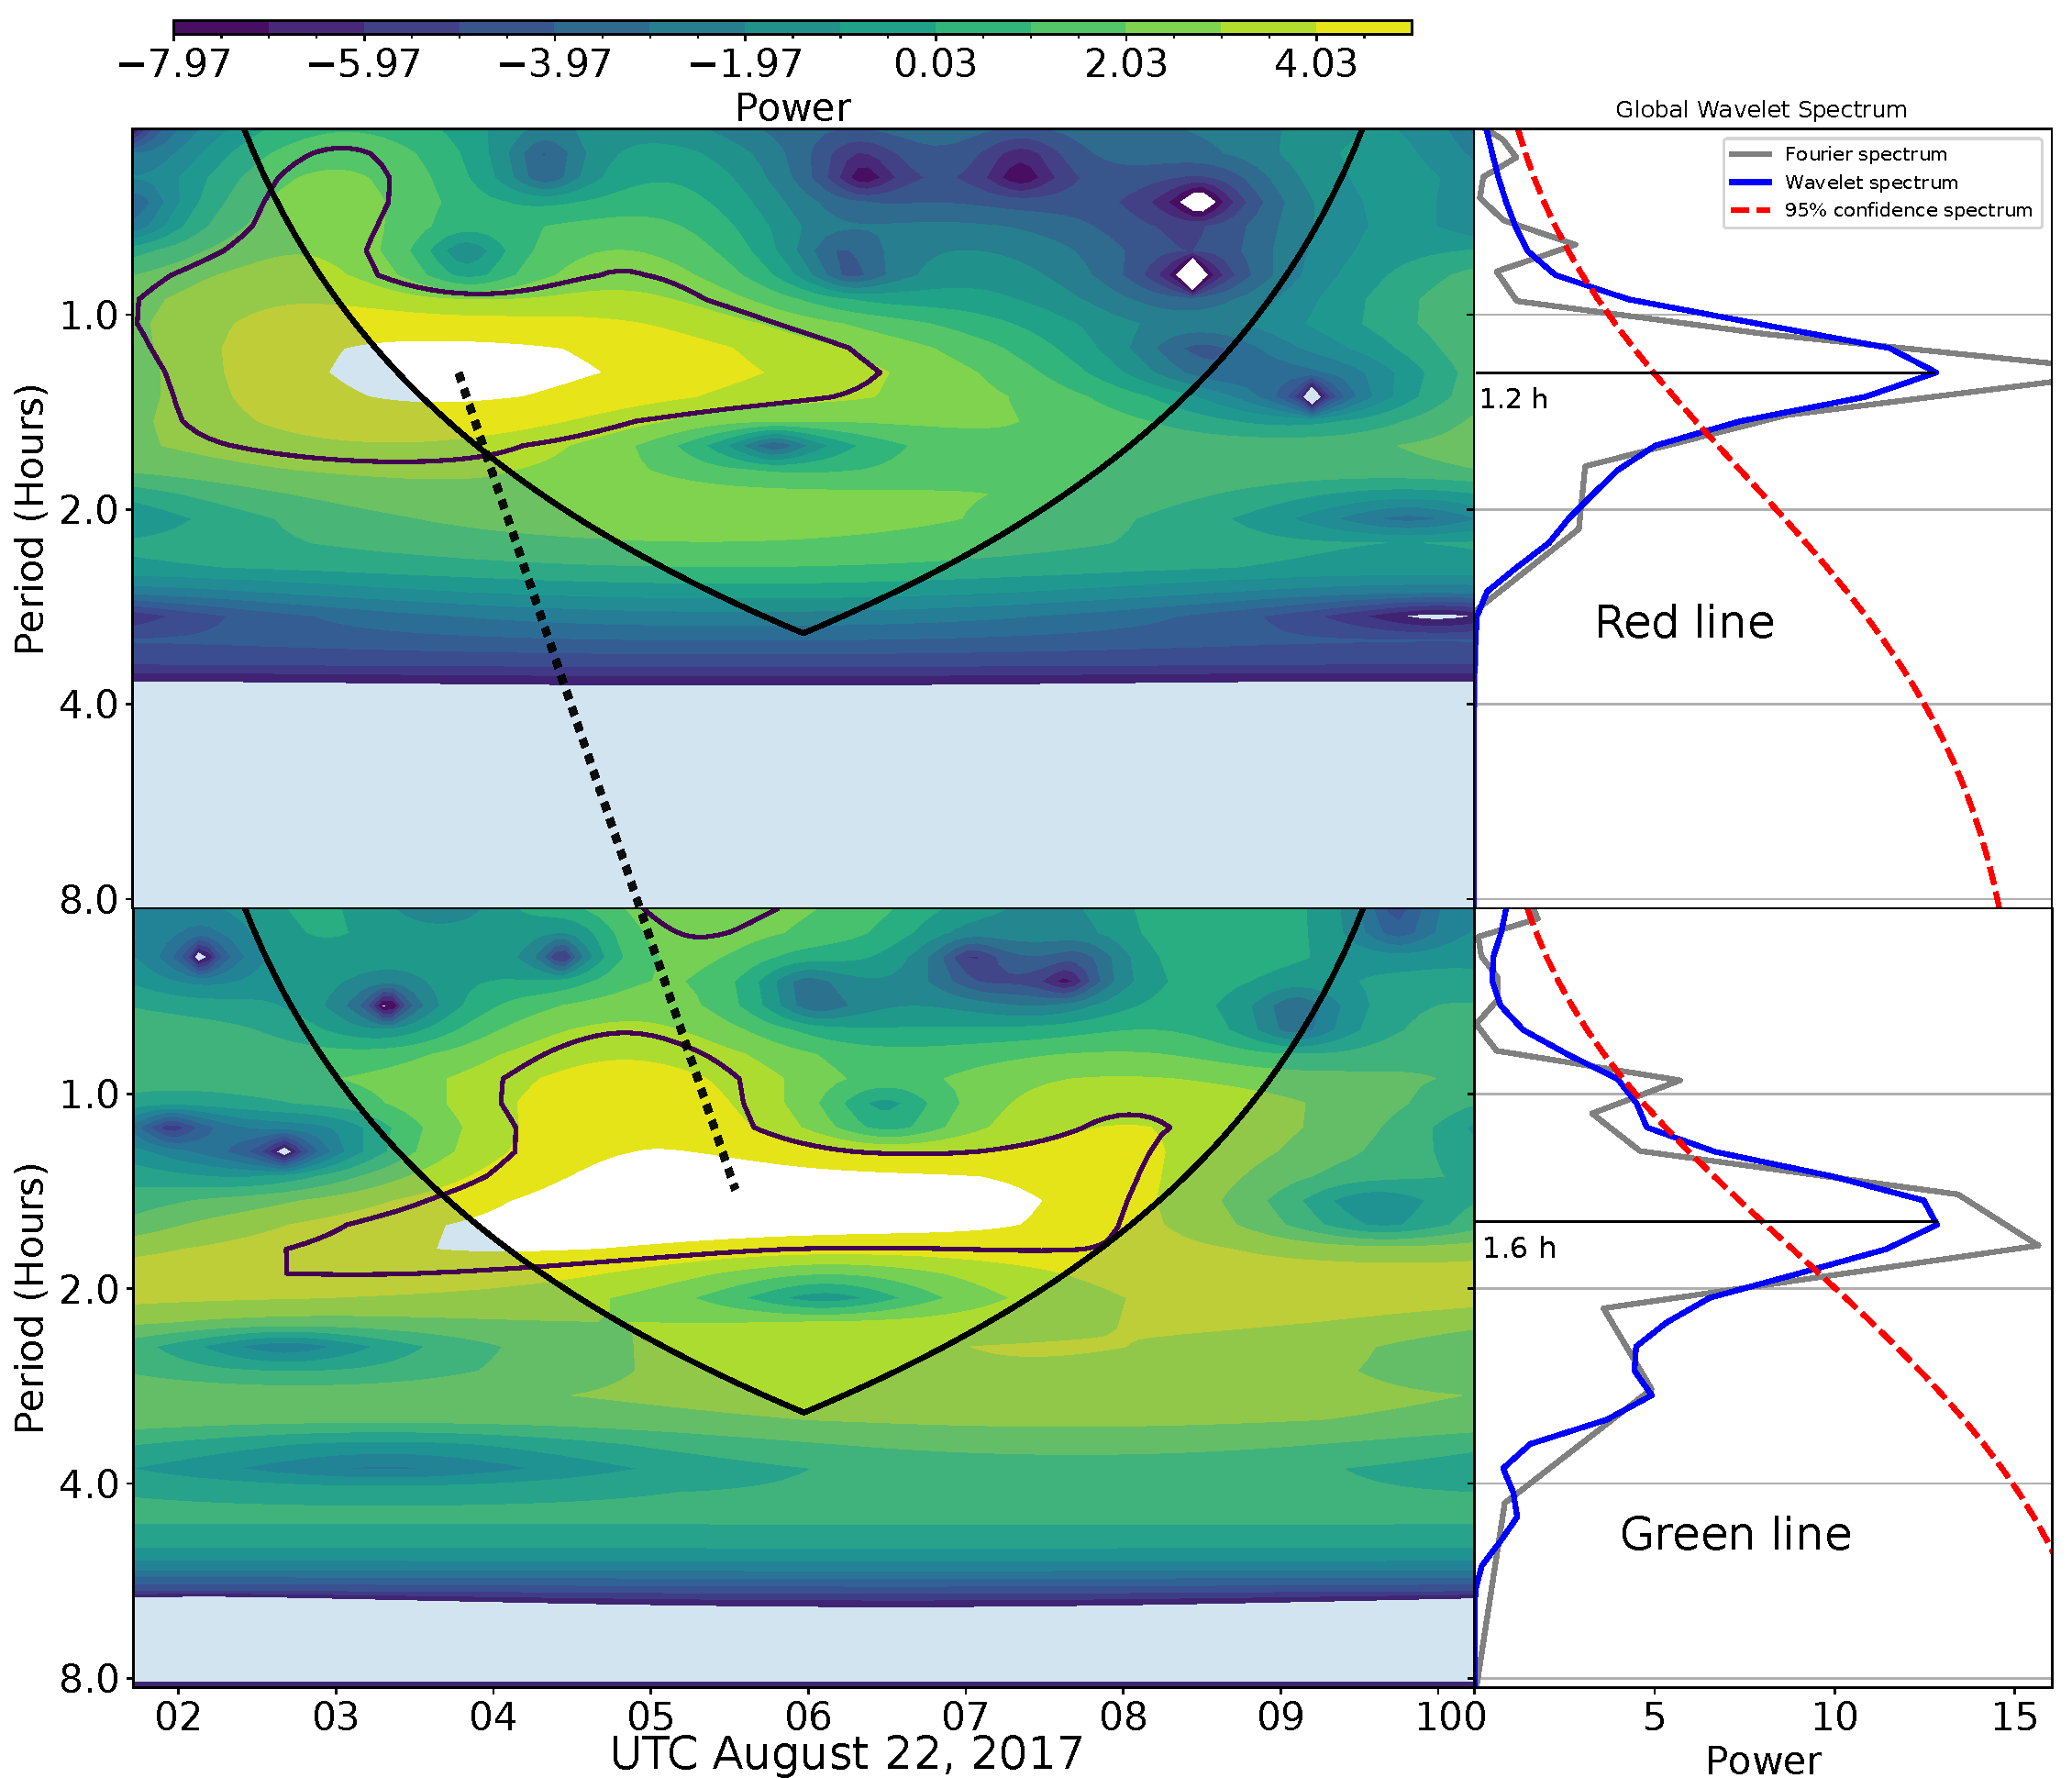
\includegraphics[width=35pc]{wavelet_red_green.pdf}
 \caption{Wavelet analysis performed on the dynamic part of the red and the green line brightnesses. The dynamic part of the brightnesses were obtained by subtracting a polynomial fit to themselves to reveal the dynamic part of the data. The dominant time period of 1.2 hour peaked around 0400 UTC for red line. Similar periodicity (1.6 hour) was seen in green line that  started around 0400 UTC and peaked around 0600 UTC. A dashed-black line is shown to highlight the shift in peak time-periods from red to the green line. Wavelet power spectrum averaged along all observation times and the corresponding Fast Fourier Transform (FFT) power spectrum and the 95$\%$ confidence interval (in red) is shown on right. 95\% + confidence-level powers on the wavelet spectra are represented by purple contours. The parabolic black line represents represents the cone of influence, below which (lightly shaded areas) the results are unreliable.}
 \label{fig:red_green_wv}
 \end{figure}
    \begin{figure}
 \centering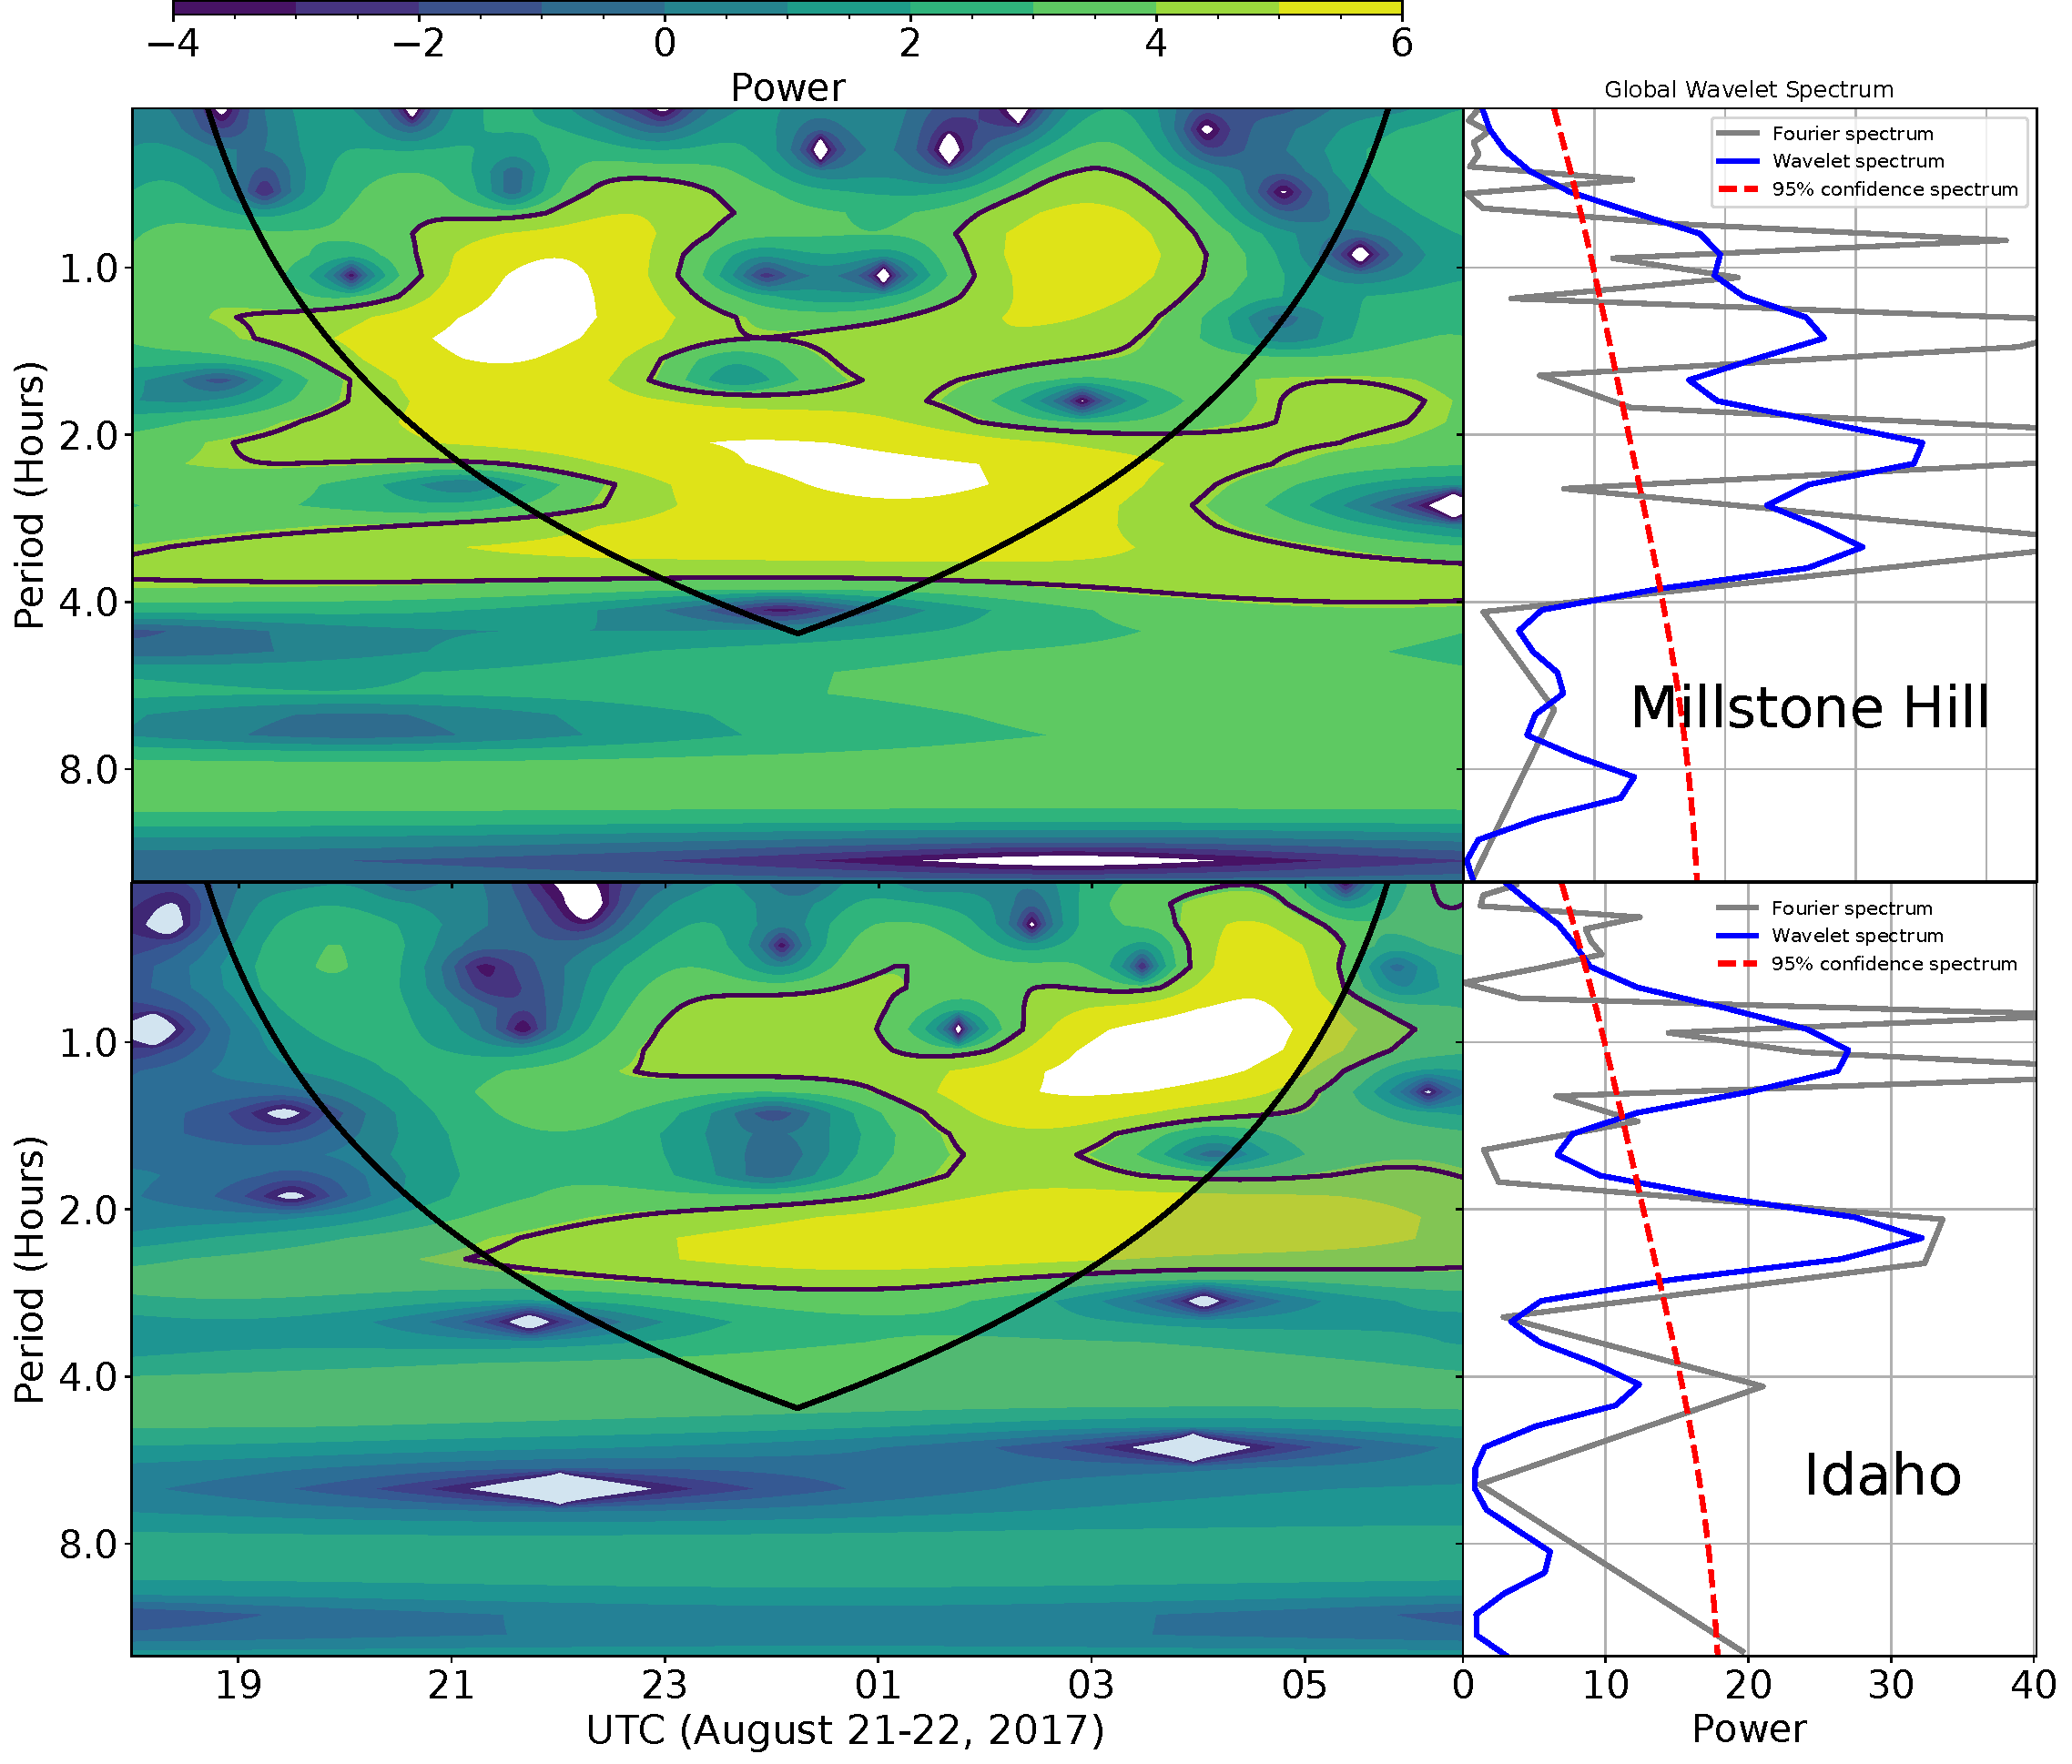
\includegraphics[width=35pc]{muf_digi_wavelet.pdf}
 \caption{Wavelet analysis performed on the dynamic part of MUF profile from the Millstone Hill (top) and  Idaho National Lab (bottom). Dominant time period of $\sim$ 1 hour around is seen at both locations at different times. Notice wavelet power spectrum with a dominant time period of $\sim$ 1 hour starting around 2100 UTC at Millstone Hill which is before the commencement of a minor geomagnetic storm and could be associated with the after effect of the eclipse. }
 \label{fig:muf_wv}
 \end{figure}
     \begin{figure}
 \centering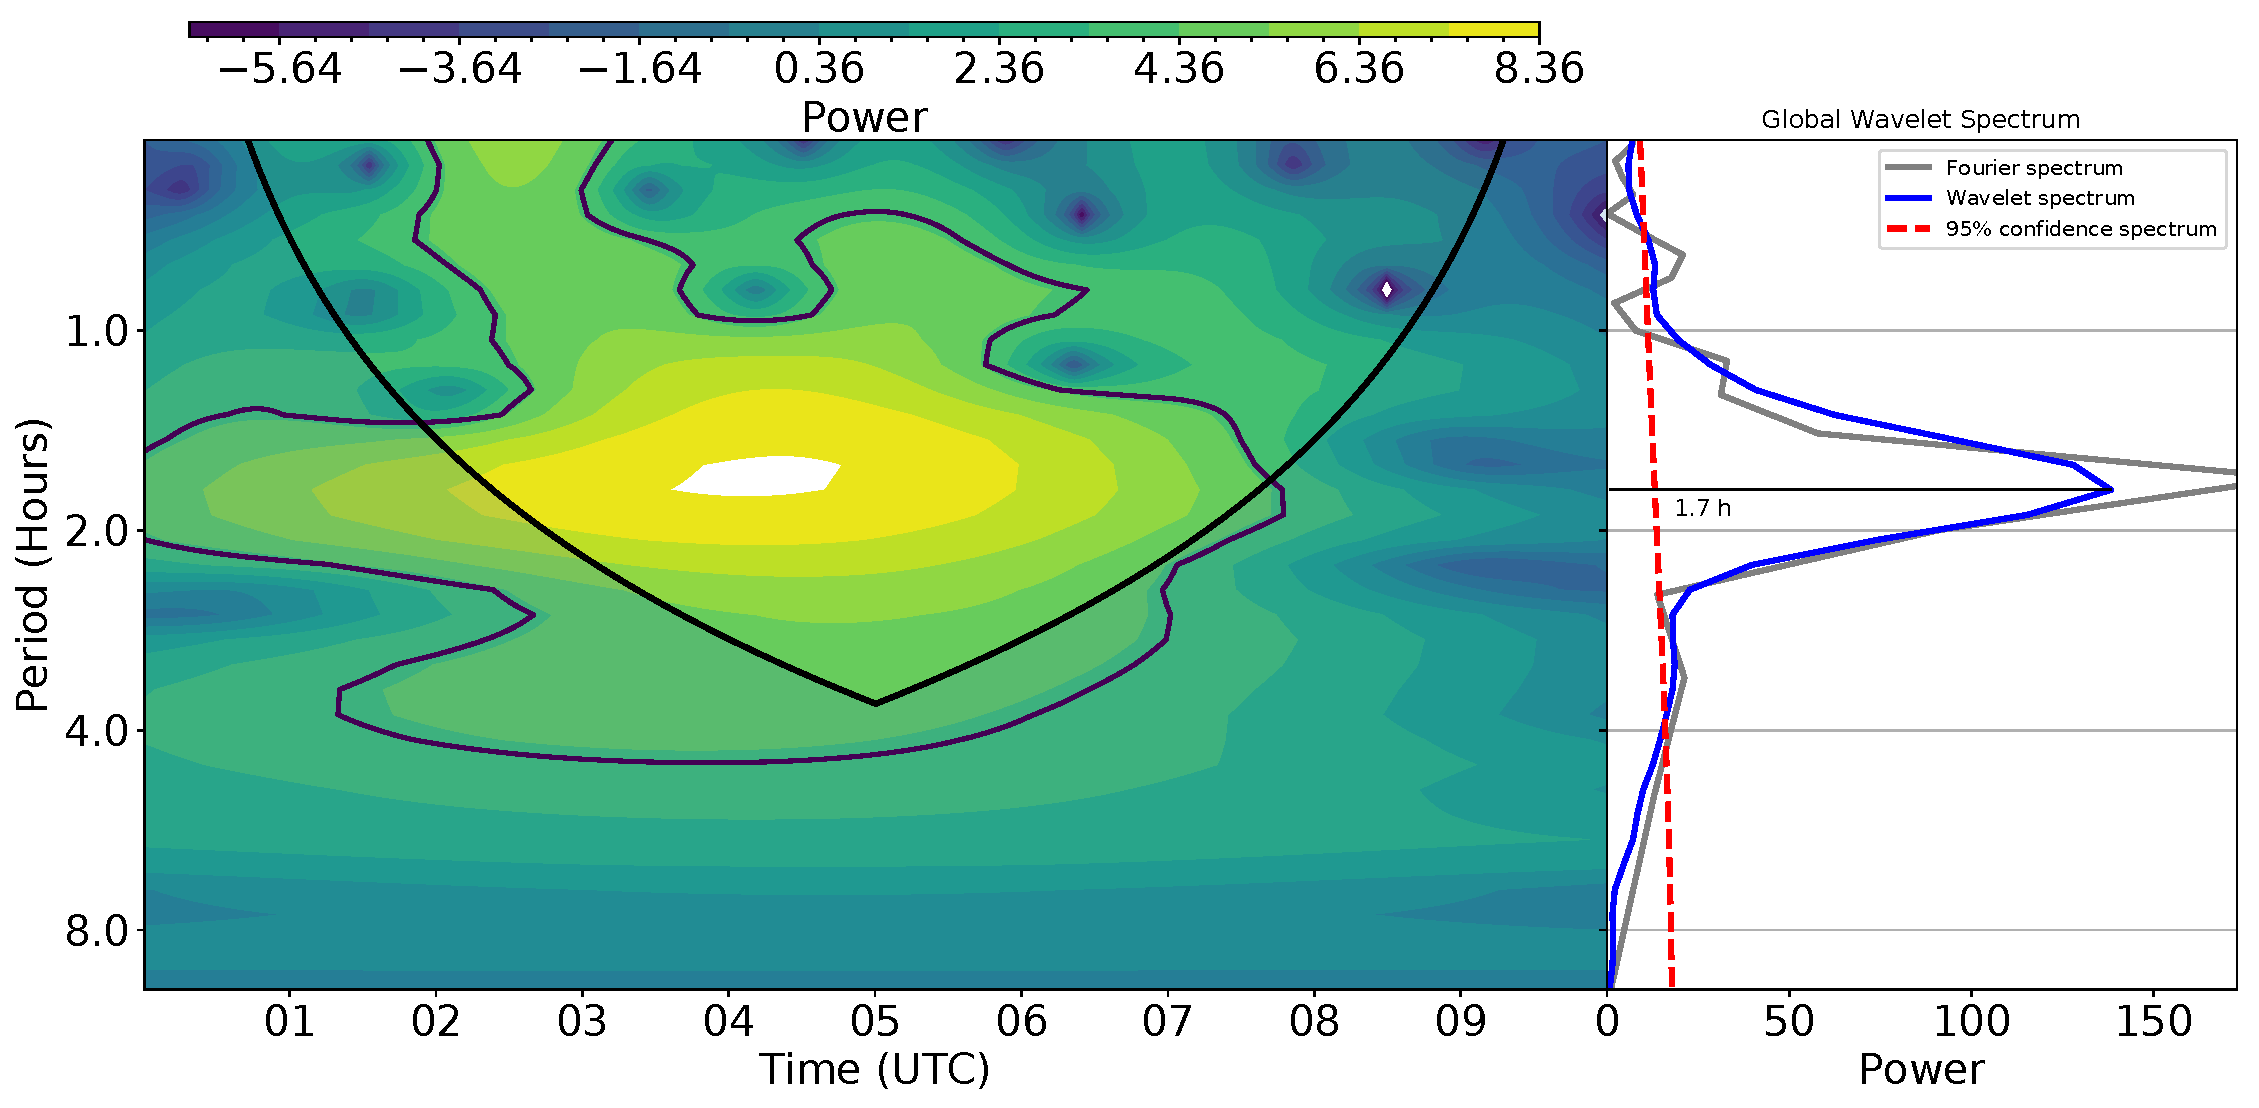
\includegraphics[width=35pc]{dtec.pdf}
 \caption{Wavelet analysis performed on the DTEC profile at Carbondale, IL from GPS TEC measurements.  Notice wavelet power spectrum with a dominant time period of 1.7 hour starting around 0400 UTC.}
 \label{fig:wav_tec}
 \end{figure} 
 
 The vertical and the the horizontal phase speeds were estimated using cross-correlation analysis. Since the red line, the green line and the DTEC profiles correlated  better from 0300 UTC to 0600 UTC (August 22, 2017) only data within these times were used. Using the difference in the peak altitude of red and green lines (250 km and 150 km, respectively) and the time delay between the signals the vertical phase speed was found to be 23 m/s. Similarly, using the distance and time delay between the DTEC measurement at 42.7$^\circ$N, 89.2$^\circ$W (not shown) and DTEC measurement at Carbondale, IL the horizontal speed was estimated to be 1500 m/s. [Note: for the horizontal speed can point to the video, 1500 m/s seems reasonable + I have not shown cross correlation plots here can decide if we need to include that too ]
 %%%
 \subsection{Effects of the Total Solar Eclipse}
While the observed TIDs were generated by geomagnetic effects, there was a total solar eclipse event eight hours earlier (August 21, 2017). The effect of a total solar eclipse on the IT system has been well-documented by recent and prior studies (see, \citet{coster_gnss_2017,mrak_eclipse_2018,liu_1998}, for example). Furthermore, MUF profiles at Idaho National Lab and Millstone Hill show perturbation even prior to the start of geomagnetically active time (Figure \ref{fig:digi}, before midnight UTC). This could potentially represent the lingering effect of the eclipse.  
%%% From Ingrid

GITM \citep{ridley_global_2006} was used to simulate the effects of the August 21, 2017 eclipse on the IT system. To do this, GITM was modified to reduce the EUV heating and ionization in the region of the moon occultation of the Earth. This was done as described by \citet{wu_gitm-data_2018}, although they used a different EUV model. The path of the eclipse was defined in Geocentric Solar Ecliptic (GSE) coordinates as a straight line in the (Y$_{GSE}$, Z$_{GSE}$)-plane, assuming X$_{GSE}$ constant. The reduction in EUV irradiance was based on the distance between each GITM grid point and the center of totality: at the center of totality, the EUV irradiance was reduced to 10\% of the normal value, which linearly increased until the edge of the occultation region was approached, after which the EUV increased exponentially back to 100\% at 3,800 km distance from the center of totality.

Two simulations were run: one with the eclipse event included and one without for comparison (the control simulation). Both simulations were otherwise set up identically. The model was run with a resolution of 0.5$^\circ$ in latitude, 2.0$^\circ$ in longitude, and $\sim$0.3 times the scale height in altitude, spanning from 100 km to approximately 600 km altitude. Observed solar wind and interplanetary magnetic field data were used to drive the high-latitude electric potential and auroral precipitation patterns. The simulations used here are the same as those analyzed by Cnossen et al. [in preparation], who describe the simulation setup in further detail. 
% The electron transport model, GLOW \citep{solomon_1988,solomon1989630,bailey2002}, was used to estimate the red and green line brightnesses based on climatological and GITM derived inputs. 
%%%%%%%%%%%%%

Figure \ref{fig:ec_ne} shows the electron density and  the thermospheric O/N$_2$ ratios estimated using GITM at 250 km, which is where the red line emission peaks, with and without the effect of the eclipse. It was seen that both electron density and the O/N$_2$ ratio were $\sim$ 10\% higher with eclipse but the time profile was very similar to the non-eclipse case. However, \citep{wu_gitm-data_2018} reported that IT system's response to the eclipse in GITM decays much more quickly than observations. Furthermore, \citet{goncharenko_mh_hill_eclipse} reported enhanced electron density (> 50-150\%) starting from 2100 UTC, August 21, 2017 to at least midnight UTC (August 22) based on radar measurements at MH hours after the eclipse.  The authors attributed this to the downward flux of plasma from the plasmasphere that was filled by upwelling of plasma immediately following the eclipse. This was not predicted by the GITM model in their study. On the other hand, 10\% increase in both O/N$_2$ ratio and N$_e$ at Carbondale, IL predicted by GITM is consistent with the qualitative enhancement in red line brightness we observed (compared to the night before, see Supplimentary information).  Thus, no conclusion on the possibility of eclipse contributing to the formation of the observed TIDs could be drawn.  
% Figure \ref{fig:ec_ne} (bottom) shows GLOW model brightness estimates using GITM inputs (both with and without eclipse's effect). The red and the green line brightnesses scaled to the climatological GLOW estimates the night before (assumed to have no disturbances) plus the climatological GLOW brightness estimates are also shown for comparison. GLOW's brightness estimates for the red line using GITM's inputs  with eclipse's effect are comparable to the data until the brightness perturbations occur ($\sim$ 0300 UTC). 
%%%%GITM model e(nhanced Ne
   \begin{figure}
 \centering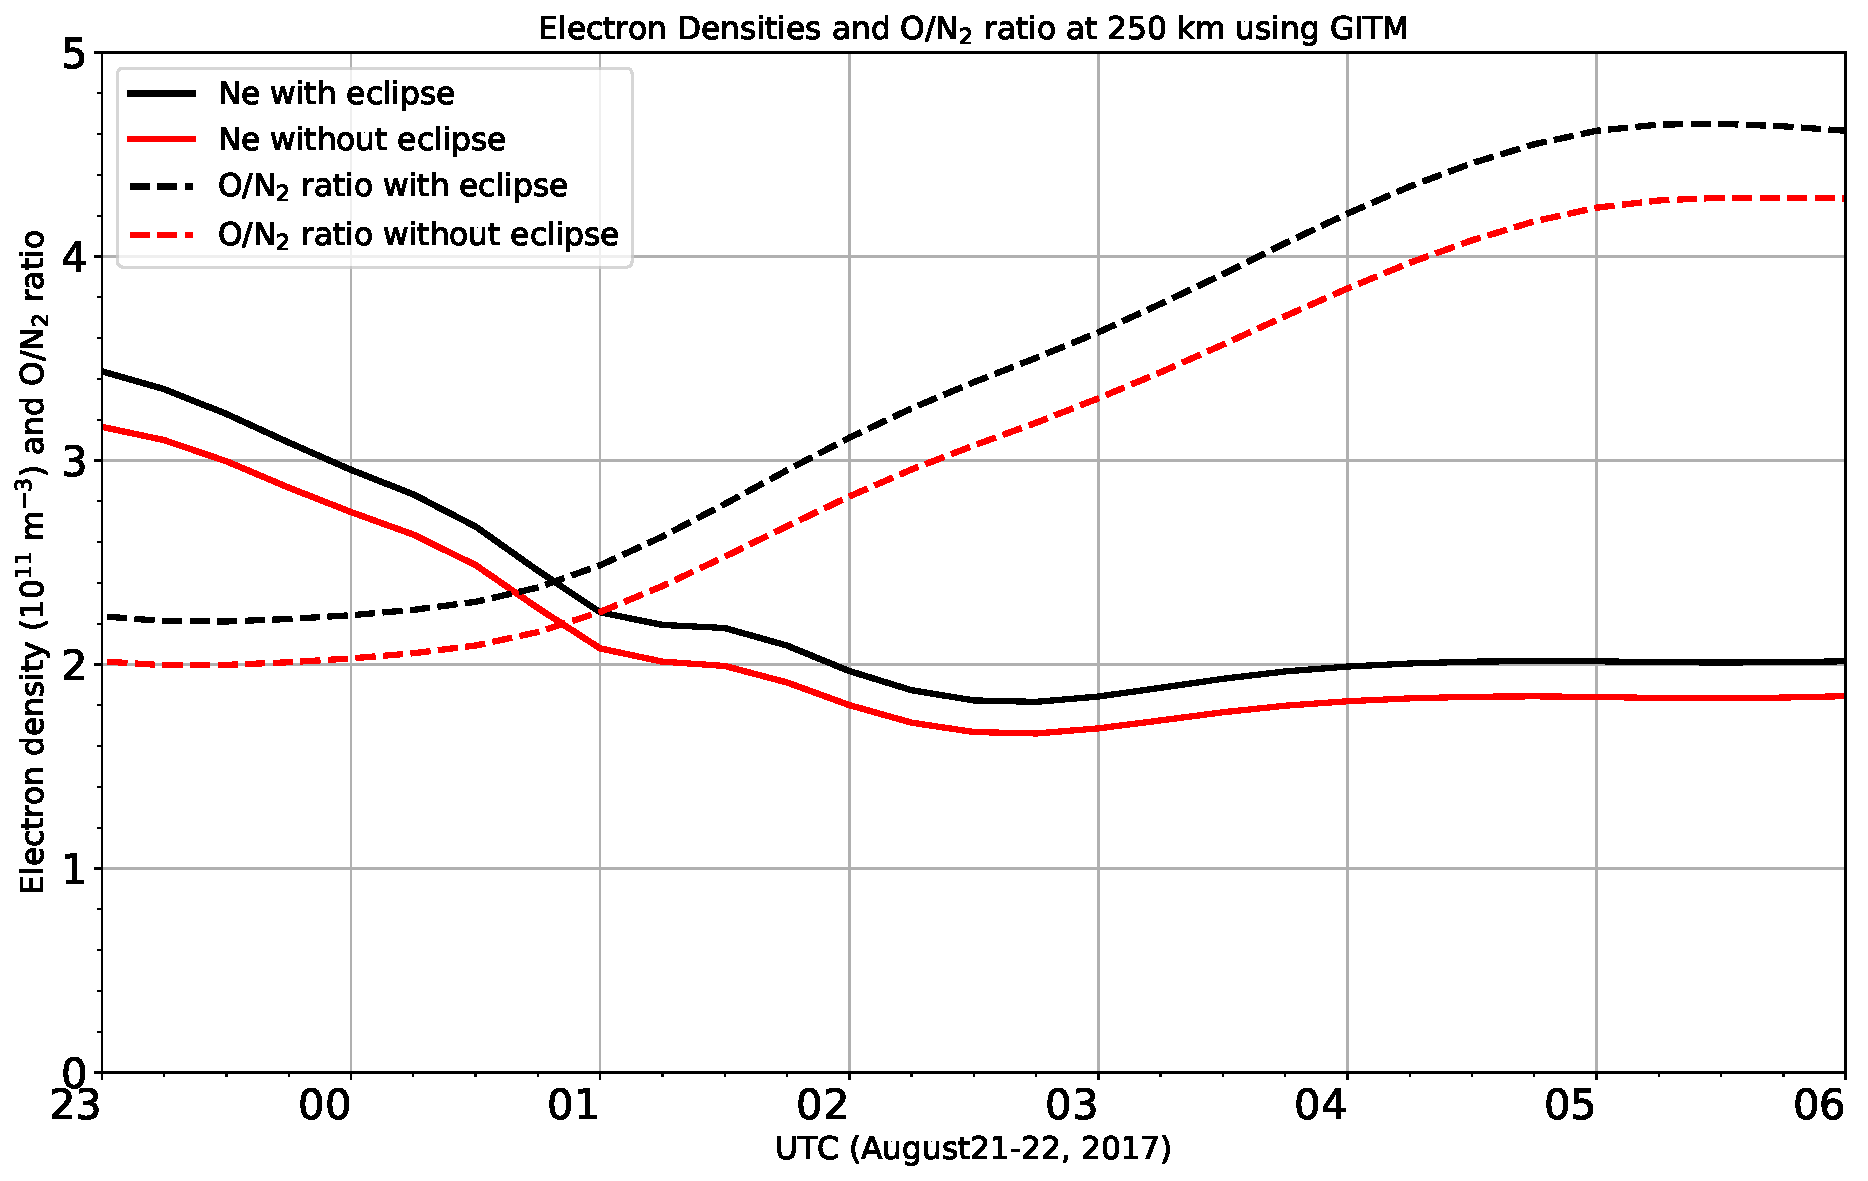
\includegraphics[width=30pc]{ec_vs_nec_tid.pdf}
 %\centering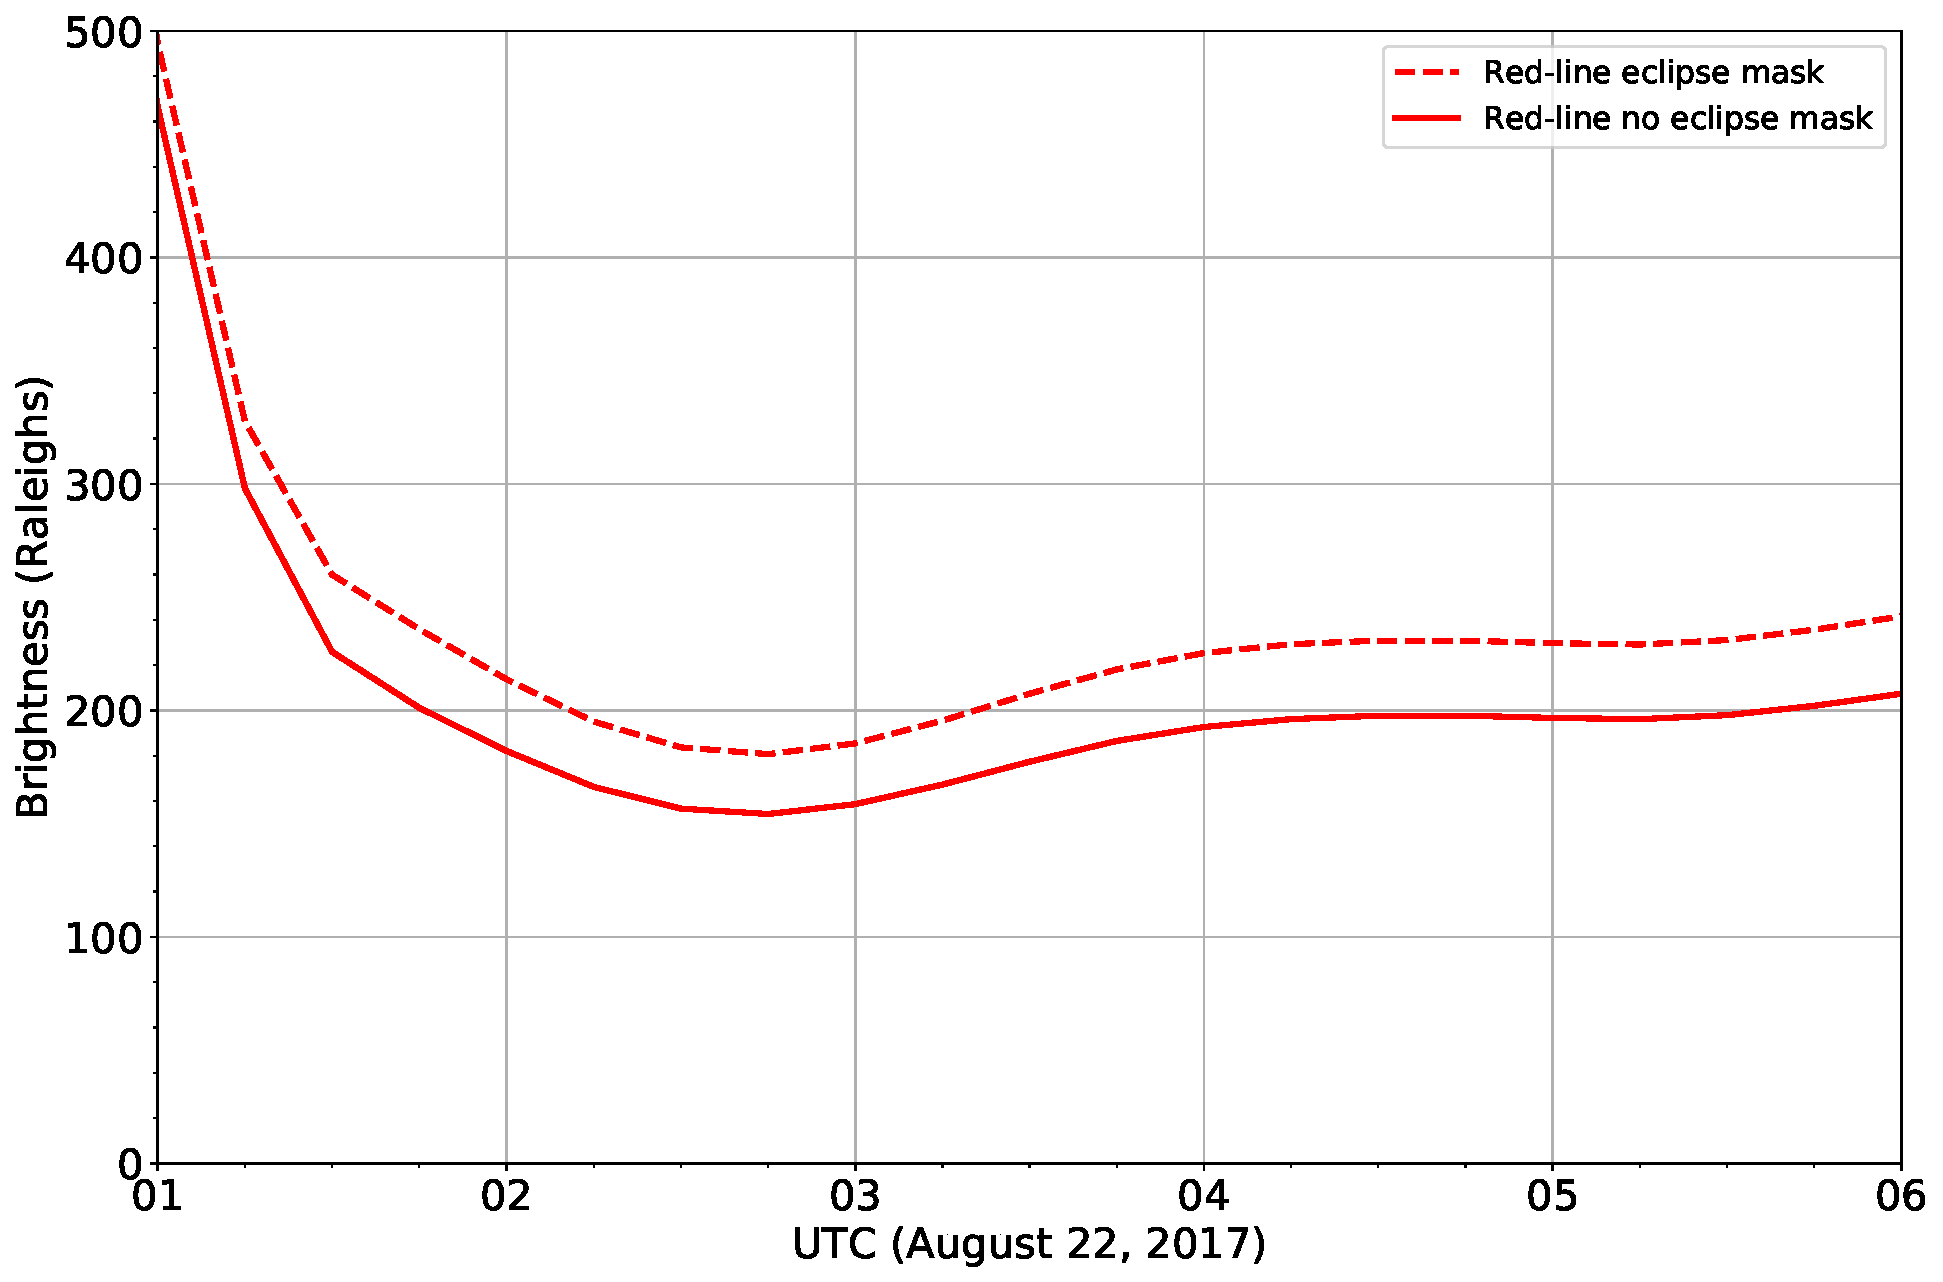
\includegraphics[width=30pc]{GITM_with_GLOW_dglow.pdf}
 \caption{ Electron densities  and the thermospheric O/N$_2$ ratio at 250 km (peak of red line emission) using an EUV mask to mimic the effect of a total solar eclipse, and normal conditions (but including geomagnetic effects) using the GITM model at Carbondale, IL. Notice that while the profiles are very similar, both electron density and the O/N$_2$ ratios are $\sim$ 10\% higher when the effects due the eclipse were considered. }
 \label{fig:ec_ne}
 \end{figure}

%This section describes the GITM model based on writeup I will get from  Dr. Cnossen.
%  Numbered lines in equations:
%  To add line numbers to lines in equations,
%  \begin{linenomath*}
%  \begin{equation}
%  \end{equation}
%  \end{linenomath*}

\section{Discussion}
[Can decide if this is necessary as I have tried to explain most things on the spot.]

\section{Summary}
We have presented observations of wave-like perturbation in red and green line brightness from ground-based optical measurements, in MUF profiles based on digisonde measurements (at two different locations), and in TEC based on GPS TEC measurements. Based on wavelet analysis, all of the measurements of similar dominant time period of $\sim$ 1-1.7 hours.  A minor geomagnetic disturbance occurred starting midnight UTC (August 22, 2017) and enhanced the auroral currents (peak AE index $\sim$ 1000 nT, see Figure \ref{fig:gindx}) potentially leading to Joule heating. We conclude that this heating expanded the IT system and triggered AGWs (and associated TIDs) propagating towards the equator. Furthermore, a total solar eclipse had occurred hours earlier over the continental USA. Previous studies have observed disturbed upper atmosphere well after from the eclipse and far away from its path (\citet{harding_nightside_eclipse,eclipse_belg}, for example). Simulations using EUV mask to mimic the lunar shadow's effect on the upper atmosphere have also predicted disturbed upper atmosphere long after the eclipse \citep{huba_drob_2017}. By using the GITM simulation, we found that preconditioning due to eclipse increased N$_e$ and O/N$_2$ ratio at 250 km $\sim$ 10 \% during the observed TID event. However, no conclusion could be drawn on if eclipse directly helped with the TIDs formation. Using cross-correlation on the red and the green line brightness profiles, the vertical phase speed was found to be 23 m/s. Similarly, using DTEC measurements at two locations the horizontal speed was estimated to be 1500 m/s.
